\chapter{Implementation}
\label{chap:implementation}

This chapter presents the implementation details of a WASI Preview 1 I2C interface designed specifically for \acrshort{wamr}, addressing the critical requirement for embedded device support in the WASI I2C standardization proposal. Building upon Friedrich's foundational work~\cite{friedrich_paper}~\cite{friedrich_impl}, this implementation establishes a comprehensive Preview 1 setup that enables resource-constrained embedded systems to participate in the I2C standardization effort.

The implementation serves as an exploration of how the WASI I2C interface could be adapted for Preview 1 environments, providing essential groundwork for the proposal's progression to the next standardization phase, which requires demonstrated compatibility with embedded device constraints.

\section{System Overview \& Architecture}
\label{sec:system-overview}

\subsection{Implementation Context and Scope}

The development effort encompasses five core implementations that collectively demonstrate Preview 1 I2C interface feasibility:

\begin{minted}{text}
    wasip1-i2c-lib/          // Manual Preview 1 bindings library
    wasip1-i2c-guest/        // Core WASM module (target: wasm32-wasip1)
    wasip2-i2c-guest/        // WASM component (target: wasm32-wasip2)
    wamr_impl/               // WAMR host runtime implementation
    wasmtime_impl/           // Wasmtime host runtime implementation
\end{minted}

\begin{figure}[h]
	\centering
	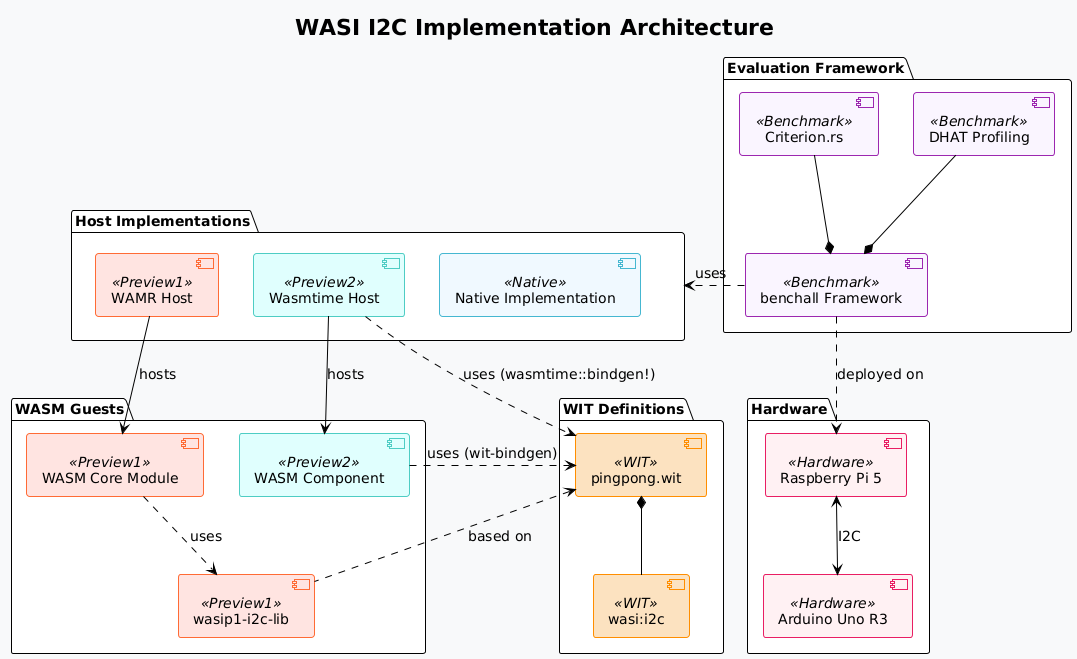
\includegraphics[width=\textwidth]{images/project schema.png}
	\caption{Overview of the project structure, showcasing the structure and interaction between different components}
	\label{fig:project_schema}
\end{figure}

All implementations in this ecosystem, including the Preview 2 component and Wasmtime host, represent original contributions developed specifically for this research. The system design enables direct comparison between Preview 1 and Preview 2 approaches while maintaining functional equivalence in I2C communication capabilities.

\subsection{I2C Interface Implementation: Simplified vs. Official Specification}

This implementation utilizes a simplified version of the WASI I2C interface rather than the complete official specification. The choice to use a reduced interface provides focus on core I2C functionality while demonstrating the essential capabilities needed for I2C communication.

Code Fragments \ref{lst:official-i2c-interface} and \ref{lst:simplified-i2c-interface} showcase the main differences between the official and the simplified interface definition. The complete definition of the interface is available in the proposal's repository~\cite{wasi_i2c_proposal}.

\begin{listing}[H]
    \begin{minted}{rust}
    interface i2c {
        // Defined types and error features
        ... 
        
        variant operation {
            read(u64),
            write(list<u8>)
        }
    
        resource i2c {
            /// Execute complex multi-operation transactions
            transaction: func(address: address, operations: list<operation>) 
                        -> result<list<list<u8>>, error-code>;
            
            /// Basic read operation
            read: func(address: address, len: u64) -> result<list<u8>, error-code>;
            
            /// Basic write operation  
            write: func(address: address, data: list<u8>) -> result<_, error-code>;
            
            /// Combined write-then-read operation
            write-read: func(address: address, write: list<u8>, read-len: u64) 
                       -> result<list<u8>, error-code>;
        }
    }
    \end{minted}
    \caption{Official WASI I2C interface specification with comprehensive transaction support}
    \label{lst:official-i2c-interface}
\end{listing}

\begin{listing}[H]
    \begin{minted}{rust}
    interface i2c {
        // Defined types and error features
        ... 
    
        resource i2c {
            /// Core read functionality
            read: func(address: address, len: u64) -> result<list<u8>, error-code>;
            
            /// Core write functionality
            write: func(address: address, data: list<u8>) -> result<_, error-code>;
        }
    }
    \end{minted}
    \caption{Simplified I2C interface providing core read and write functionality}
    \label{lst:simplified-i2c-interface}
\end{listing}

The simplified interface excludes the transaction and write-read methods, concentrating on the fundamental read and write operations that form the basis of I2C communication. This approach provides sufficient functionality for validating the Preview 1 adaptation approach while reducing implementation complexity. The error handling remains comprehensive, preserving all essential I2C protocol error conditions and their semantic information.

\subsection{Pingpong World and WIT Structure Organization}

The pingpong world serves as the primary application interface that demonstrates the use of the (simplified) I2C interface. This world defines the contract between guest components and their host environment, establishing the essential imports and exports needed for I2C communication validation.

\begin{listing}[H]
    \begin{minted}{rust}
    // Pingpong world using simplified I2C interface
    package my:pingpong;
    
    world pingpong {
        import wasi:i2c/i2c;
        use wasi:i2c/i2c.{i2c};
    
        import get-i2c-bus: func() -> i2c;
        export run: func();
    }
    \end{minted}
    \caption{Pingpong world definition demonstrating I2C resource acquisition and application entry point}
    \label{lst:pingpong-world}
\end{listing}

The pingpong world imports the simplified I2C interface and provides a `get-i2c-bus` function that returns an I2C resource. The world exports a single `run` function that serves as the application's entry point, enabling straightforward validation of the complete I2C communication cycle.

The WIT directory structure follows the standard organization pattern established by the component model ecosystem:

\begin{minted}{text}
wit/
    pingpong.wit              // Main world definition
    deps/
        wasi-i2c/
            i2c.wit           // Simplified I2C interface
            world.wit         // I2C world imports
\end{minted}

The `deps/wasi-i2c/` directory contains the simplified I2C interface definition along with its world imports. The simplified version has no need for the additional delay.wit and is therefore removed from the directory and the world.wit imports. This structure enables both guest and host implementations to reference the same interface definitions, ensuring consistency across the entire ecosystem.

\subsection{Technical Environment}

The implementation targets the following runtime environment specifications:

\begin{itemize}
    \item \textbf{WAMR Rust SDK Version}: v1.1.0 (uses WAMR Version 2.1.2)
    \item \textbf{Wasmtime Version}: v35.0.0
    \item \textbf{Rust Toolchain}: 1.88.0 with \texttt{wasm32-wasip1} and \texttt{wasm32-wasip2} targets
    \item \textbf{Target Architecture}: ARM64 (aarch64-unknown-linux-musl) for Raspberry Pi deployment
    \item \textbf{Component Tooling}: \texttt{cargo-component} v0.21.1 for Preview 2 builds
\end{itemize}

\subsection{Preview 1 vs Preview 2 Architectural Differences}

The fundamental challenge lies in adapting Preview 2's sophisticated resource-based component model to Preview 1's minimalist function-based interface system. This adaptation requires careful consideration of how high-level abstractions can be preserved while working within Preview 1's limited type system.

\begin{listing}[H]
    \begin{minted}{rust}
    // Preview 2: Resource-based approach with automatic lifecycle management
    world pingpong {
        // Resource management provided by Runtime
        import wasi:i2c/i2c;    // Functionality imported as dependency
        export run: func();     // Guest entry point
    }
    
    // Preview 1: Function-based approach requiring manual resource management
    world wasip1-pingpong {
        import host_open: func() -> u32;            // Resource creation
        import host_write: func(handle: u32, addr: u16, len: usize, offset: usize) -> u8;                                     // Resource functionality
        import host_read: func(handle: u32, addr: u16, len: usize, offset: usize) -> u8;                                     // Resource functionality
        import host_close: func(handle: u32);       // Resource destruction
        export run: func();                         // Guest entry point
    }
    \end{minted}
    \caption{Architectural comparison only meant for highlighting semantic gap between Preview versions and never actually used.}
    \label{lst:preview-comparison}
\end{listing}

Preview 2's component model provides automatic resource lifecycle management, type-safe binding generation, and sophisticated error handling mechanisms. In contrast, Preview 1 requires manual implementation of all these features through carefully designed function interfaces and explicit resource tracking systems.

\section{Canonical ABI Adaptation and Design Choices}
\label{sec:canonical-abi-adaptation}

\subsection{Canonical ABI Compatibility and Implementation Options}

The WebAssembly Component Model defines a Canonical Application Binary Interface (ABI) that specifies how WIT definitions are translated to bits and bytes for inter-component communication. This ABI provides standardized mechanisms for passing complex data structures, managing resources, and handling errors between WebAssembly components and their host environments.

\subsection{Context-Driven ABI Design Decisions}

Rather than indicating a limitation or incompatibility, the departure from strict Canonical ABI compliance represents a deliberate design choice based on the specific context and constraints of embedded I2C communication. Understanding the application domain enables targeted optimizations that would not be possible with a generic ABI approach.

\textbf{Error Handling Optimization}: The Canonical ABI represents errors using a discriminated union approach, where the error type discriminant and error-specific data (such as NoAcknowledgeSource) would be stored in separate fields, similar to C union structures. The Preview 1 implementation consolidates this information into a single byte using bit manipulation, providing an errno-like interface that reduces memory usage and simplifies error propagation in resource-constrained environments.

\textbf{Memory Management Adaptation}: While the Canonical ABI specifies host-managed memory allocation as the standard, this implementation makes use of guest-managed allocations to showcase the flexibility of Preview 1.

\subsection{Trade-offs of Context-Specific Optimization}

\textbf{Advantages of Custom Approach}:
\begin{itemize}
    \item \textbf{Embedded Optimization}: Targeted optimizations for I2C communication patterns reduce memory usage and improve predictability for embedded deployment scenarios.
    \item \textbf{Simplified Error Model}: The errno-style error reporting aligns with embedded programming conventions and reduces complexity in error handling logic.
    \item \textbf{Resource Efficiency}: Compact error encoding and optimized memory patterns minimize overhead in resource-constrained environments.
    \item \textbf{Deterministic Behavior}: Context-specific optimizations enable more predictable performance characteristics suitable for real-time embedded applications.
\end{itemize}

\textbf{Disadvantages of Deviation from Standards}:
\begin{itemize}
    \item \textbf{Reduced Interoperability}: Custom ABI choices limit compatibility with generic WebAssembly tooling and component model infrastructure.
    \item \textbf{Development Overhead}: Manual implementation requires more effort compared to automatic Canonical ABI generation.
    \item \textbf{Maintenance Complexity}: Custom ABI implementations require manual updates when interface specifications change.
    \item \textbf{Limited Reusability}: Context-specific optimizations may not transfer to other use cases or interface types.
\end{itemize}

The decision to deviate from the Canonical ABI represents a conscious trade-off between universal compatibility and context-specific optimization. While the Canonical ABI could be fully implemented for this use case, the specific constraints and patterns of embedded I2C communication justify targeted optimizations that provide benefits in the target deployment environment.

\section{WASI Preview 1 Bindings Implementation}
\label{sec:wasip1-bindings}

\subsection{Conditional Compilation Architecture}

The \texttt{wasip1-i2c-lib} crate represents the core innovation of this implementation, providing a carefully architected bridge between the high-level semantics defined in WIT specifications and the low-level function interfaces required by Preview 1. The library employs conditional compilation to support both guest and host use cases without imposing unnecessary dependencies on either environment.

\begin{listing}[H]
    \begin{minted}{toml}
    # wasip1-i2c-lib/Cargo.toml
    [features]
    default = []        # Common type definitions and utility only
    guest-utils = []    # Enables guest-specific resource management functionality
    
    [lib]
    crate-type = ["lib"]
    \end{minted}
    \caption{Feature flag configuration enabling flexible deployment across guest and host environments}
    \label{lst:conditional-compilation}
\end{listing}

The \texttt{guest-utils} feature flag determines whether guest-specific functionality is compiled, allowing the same codebase to serve multiple deployment scenarios. When enabled, the library provides high-level resource management abstractions for guest modules. When disabled, it provides only the type definitions and utility functions needed by host implementations.

\subsection{Type System Design and WIT Compatibility}

The type system design preserves the semantic richness of WIT specifications while adapting to Preview 1's constraints. Each WIT type has a corresponding Preview 1 representation that maintains the same information content but fits within the limitations of primitive parameter passing.

\begin{listing}[H]
    \begin{minted}{rust}
    // wasip1-i2c-lib/src/common.rs
    pub type I2cAddress = u16;
    pub type I2cResourceHandle = u32;
    
    #[repr(u8)]
    #[derive(Debug, Clone, Copy)]
    pub enum NoAcknowledgeSource {
        Address,
        Data,
        Unknown,
    }
    
    #[derive(Debug, Clone)]
    pub enum ErrorCode {
        None,
        Bus,
        ArbitrationLoss,
        NoAcknowledge(NoAcknowledgeSource),
        Overrun,
        Other,
    }
    \end{minted}
    \caption{Type definitions maintaining semantic compatibility with WIT specifications while using primitive representations}
    \label{lst:type-definitions}
\end{listing}

\subsection{Error Encoding and Recovery Mechanisms}

The error handling system represents the most sophisticated aspect of the type translation challenge. WIT's rich error types are encoded into single-byte values for efficiency, using a carefully designed bit-packing scheme that preserves all semantic information. An additional \texttt{ErrorCode::None} was added to support the earlier discussed errno-style reporting for when the call is successful.

\begin{listing}[H]
    \begin{minted}{rust}
    impl ErrorCode {
        /// Encode error into Preview 1 compatible byte representation
        pub fn lower(&self) -> u8 {
            match self {
                ErrorCode::None => 0b000_00000,
                ErrorCode::Bus => 0b001_00000,
                ErrorCode::ArbitrationLoss => 0b010_00000,
                ErrorCode::NoAcknowledge(source) => {
                    let no_ack_bits = source.lower();
                    0b011_00000 | no_ack_bits  // Combine error type with source info
                }
                ErrorCode::Overrun => 0b100_00000,
                ErrorCode::Other => 0b101_00000,
            }
        }
    
        /// Decode Preview 1 byte representation back to rich error type
        pub fn lift(val: u8) -> ErrorCode {
            let error_type = val >> 5;           // Extract first 3 bits
            let error_variant = val & 0b000_11111; // Extract last 5 bits
            
            match error_type {
                0 => ErrorCode::None,
                1 => ErrorCode::Bus,
                2 => ErrorCode::ArbitrationLoss,
                3 => ErrorCode::NoAcknowledge(
                        NoAcknowledgeSource::lift(error_variant)
                    ),
                4 => ErrorCode::Overrun,
                _ => ErrorCode::Other,
            }
        }
    }
    \end{minted}
    \caption{Bidirectional error encoding scheme preserving WIT semantic information within Preview 1 constraints}
    \label{lst:error-encoding}
\end{listing}

This encoding scheme utilizes the upper three bits for error type classification and the lower five bits for error-specific information, ensuring that no semantic information is lost during the Preview 1 translation process.

\subsection{Guest-Side Resource Management}

The guest-side resource management system provides lifecycle management based on \acrfull{raii}. It mirrors the automatic resource handling available in Preview 2 components:

\begin{listing}[H]
    \begin{minted}{rust}
    // wasip1-i2c-lib/src/guest.rs
    #[link(wasm_import_module = "host")]
    unsafe extern "C" {
        #[link_name = "host_open"]
        unsafe fn host_open() -> I2cResourceHandle;
        #[link_name = "host_read"]
        unsafe fn host_read(_: I2cResourceHandle, _: I2cAddress, 
                           _: usize, _: *mut u8) -> u8;
        #[link_name = "host_write"]
        unsafe fn host_write(_: I2cResourceHandle, _: I2cAddress, 
                            _: usize, _: *const u8) -> u8;
        #[link_name = "host_close"]
        unsafe fn host_close(_: I2cResourceHandle);
    }
    
    #[repr(transparent)]
    pub struct I2cResource {
        handle: I2cResourceHandle,
    }

    impl I2cResource {
        /// Create new I2C resource, acquiring handle from host
        pub fn new() -> Self {
            let handle = unsafe { host_open() };
            Self { handle }
        }
    }
    
    impl Drop for I2cResource {
        /// Automatic resource cleanup ensuring no handle leaks
        fn drop(&mut self) {
            unsafe { host_close(self.handle); }
        }
    }
    \end{minted}
    \caption{Foreign function interface declarations and \acrshort{raii}-based resource management implementation providing automatic lifecycle control for I2C handles}
    \label{lst:guest-ffi-declarations}
\end{listing}

\begin{listing}[H]
    \begin{minted}{rust}
    // wasip1-i2c-lib/src/guest.rs
    impl I2cResource {
        /// Perform I2C write operation with comprehensive error handling
        pub fn write(&self, address: I2cAddress, data: &[u8]) -> Result<(), ErrorCode> {
            let result = unsafe {
                host_write(self.handle, address, data.len(), data.as_ptr())
            };
            
            match ErrorCode::lift(result) {
                ErrorCode::None => Ok(()),
                error => Err(error),
            }
        }
    
        /// Perform I2C read operation returning allocated data buffer
        pub fn read(&self, address: I2cAddress, len: usize) 
                   -> Result<alloc_crate::vec::Vec<u8>, ErrorCode> {
            let mut read_buffer: Vec<core::mem::MaybeUninit<u8>> = 
                Vec::with_capacity(len);
    
            let host_res = unsafe {
                read_buffer.set_len(len);
                host_read(self.handle, address, len, 
                         read_buffer.as_mut_ptr() as *mut u8)
            };
    
            match ErrorCode::lift(host_res) {
                ErrorCode::None => Ok(unsafe { core::mem::transmute(read_buffer) }),
                error => Err(error),
            }
        }
    }
    \end{minted}
    \caption{Function bindings required by a I2C resource, with ``\texttt{read}'' showcasing guest-managed heap allocation}
    \label{lst:guest-resource-management}
\end{listing}

The \acrshort{raii} pattern ensures that I2C resources are automatically cleaned up when they go out of scope, preventing resource leaks that could be particularly problematic in embedded environments where resource recovery might be limited.

\section{Guest Implementations}
\label{sec:guest-implementations}

\subsection{Preview 1 Module}

The Preview 1 guest implementation (\texttt{wasip1-i2c-guest}) represents a carefully optimized approach designed specifically for resource-constrained embedded environments. This implementation prioritizes minimal binary size and runtime overhead while maintaining full functional compatibility with the I2C interface specification.

\subsubsection{No-Standard Library Configuration and Binary Size Impact}

The decision to use \texttt{\#![no\_std]} fundamentally impacts both the implementation approach and the resulting binary characteristics. This configuration eliminates the standard library's substantial memory footprint and complex runtime dependencies, resulting in significantly smaller WebAssembly modules more suitable for embedded deployment.

\begin{listing}[H]
    \begin{minted}{rust}
    // wasip1-i2c-guest/src/lib.rs (essential structure)
    #![no_std]
    #![no_main]
    
    use wasip1_i2c_lib::{common::I2cAddress, guest::I2cResource};
    
    extern crate alloc;
    use lol_alloc::{AssumeSingleThreaded, FreeListAllocator};
    
    #[global_allocator]
    static ALLOCATOR: AssumeSingleThreaded<FreeListAllocator> = unsafe {
        AssumeSingleThreaded::new(FreeListAllocator::new())
    };
    
    use core::panic::PanicInfo;
    #[panic_handler]
    fn panic(_info: &PanicInfo) -> ! {
        loop {}
    }
    \end{minted}
    \caption{Essential infrastructure for no\_std WebAssembly module requiring explicit allocator and panic handler provision}
    \label{lst:no-std-infrastructure}
\end{listing}

The \texttt{no\_std} configuration requires explicit provision of memory allocation and panic handling mechanisms that are normally provided by the standard library. The choice of \texttt{lol\_alloc} reflects embedded systems requirements where traditional heap allocators may be inappropriate due to their memory overhead or real-time characteristics.

\begin{listing}[H]
    \begin{minted}{rust}
    // wasip1-i2c-guest/src/lib.rs (main functionality)
    #[unsafe(no_mangle)]
    pub extern "C" fn _start() {
        let data = [0x68u8, 0x65, 0x6c, 0x6c, 0x6f]; // ASCII "hello"
        let slave_addr: I2cAddress = 0x0009;
        let device = I2cResource::new();
        let _ = device.write(slave_addr, &data);
        let _ = device.read(slave_addr, data.len());
    }
    \end{minted}
    \caption{Complete I2C ping-pong implementation demonstrating resource creation, bidirectional communication, and automatic cleanup}
    \label{lst:preview1-main-functionality}
\end{listing}

The resulting binary size demonstrates the effectiveness of this approach: the optimized Preview 1 module compiles to 4.8KB, compared to a significantly larger binary of 38KB that results from standard library inclusion.

\subsubsection{Memory Allocation Strategy: Guest-Managed vs Host-Managed Heap}

The implementation utilizes guest-managed heap allocation, representing an experimental departure from WAMR's default configuration and the Canonical ABI's specification for host-managed memory allocation. This design choice was more experimental and allowed for insights into the different WAMR Heap strategies. 

WAMR supports multiple heap management approaches~\cite{wamr_heaps}, each with distinct characteristics and use cases:

\begin{itemize}
    \item \textbf{WASI Heap}: Created when modules are built with WASI-LIBC, managed by the wasi-libc memory allocator. Also used by the host to allocate memory in the linear memory of the guest, when the guest module exports malloc/free functions.
    \item \textbf{Host-Managed Heap}: Created and managed by WAMR's embedded memory system (ems) allocator. The host runtime controls all memory allocation decisions and provides memory to the guest on request.
\end{itemize}

The \textbf{Canonical ABI} specification recommends \textbf{host-managed memory allocation} for several reasons: enhanced security through centralized memory control, improved resource monitoring capabilities, and simplified garbage collection integration. Host-managed approaches provide the runtime with complete visibility into memory usage patterns and enable sophisticated memory protection mechanisms.

\textbf{Rationale for Guest-Managed Allocation}: The decision to implement guest-managed heap allocation was driven by the specific characteristics of I2C read operations and experimental objectives rather than inherent performance benefits:

\begin{itemize}
    \item \textbf{Predictable Buffer Sizing}: I2C read operations require the guest to specify the expected number of bytes in advance. Guest-managed allocation allows the buffer to be pre-allocated based on this known size before initiating the host function call.
    \item \textbf{Error Handling Considerations}: When I2C operations fail, guest-managed allocation results in pre-allocated buffers that cannot be used, representing wasted allocation effort. This trade-off was accepted to explore the guest-managed approach.
    \item \textbf{Implementation Simplicity}: For the specific case of I2C communication, guest-managed allocation simplifies the host-side implementation by eliminating the need for complex memory allocation coordination.
\end{itemize}

The pure experimental nature of this choice provides valuable insights into the flexibility of Preview 1 memory management strategies while maintaining compatibility with the broader I2C interface semantics.

\subsection{Preview 2 Component: Automated Binding Generation}

The Preview 2 implementation (\texttt{wasip2-i2c-guest}) showcases the sophisticated automation capabilities of the component model while serving as a functional reference implementation.

\subsubsection{Component Model Integration and Toolchain Requirements}

The Preview 2 implementation utilizes \texttt{cargo-component}, a specialized build tool that extends Cargo's functionality to support WebAssembly component generation with automatic WIT binding creation~\cite{cargo_component_git}. This tool represents a vision of the future where WASI dependencies can be specified directly in Cargo.toml files, similar to how traditional Rust crates are managed today.

\begin{listing}[H]
    \begin{minted}{rust}
    // wasip2-i2c-guest/src/lib.rs
    #[allow(warnings)]
    mod bindings;
    
    use bindings::Guest;
    use crate::bindings::get_i2c_bus;
    
    struct PingPongComponent;
    
    impl Guest for PingPongComponent {
        fn run() {
            let dev = get_i2c_bus();
            let _ = dev.write(0x09, &[0x68, 0x65, 0x6c, 0x6c, 0x6f]);
            let _ = dev.read(0x09, 5);
        }
    }
    
    bindings::export!(PingPongComponent with_types_in bindings);
    \end{minted}
    \caption{Preview 2 component implementation leveraging automatic binding generation via cargo-component toolchain}
    \label{lst:preview2-guest}
\end{listing}

The \texttt{cargo-component} tool simulates a future ecosystem where WebAssembly components can declare their WASI interface dependencies in the same declarative manner as traditional Rust dependencies. This approach eliminates the need for manual binding generation and provides automatic type safety guarantees between component interfaces.

\begin{listing}[H]
\begin{minted}[breaklines]{toml}
# wasip2-i2c-guest/Cargo.toml (component configuration)
[package.metadata.component]
package = "my:pingpong"

[package.metadata.component.target]
path = "../wit"
world = "pingpong"

[package.metadata.component.target.dependencies]
"wasi:i2c" = { path = "../wit/deps/wasi-i2c" }
\end{minted}
\caption{Component metadata enabling automatic WIT binding generation and dependency management through \texttt{cargo-component}}
\label{lst:component-config}
\end{listing}

The component configuration metadata demonstrates how WASI interfaces could be managed as first-class dependencies in the Rust ecosystem. The `package.metadata.component.target.dependencies` section allows developers to specify WASI interfaces in the same way they would specify traditional crate dependencies, with path-based or registry-based resolution. This approach provides a foundation for a future where WASI interfaces are distributed and versioned through package registries, enabling robust dependency management for WebAssembly components.

\subsubsection{Standard Library Dependency Constraints}

Unlike the Preview 1 implementation, Preview 2 components cannot utilize \texttt{\#![no\_std]} configuration due to fundamental dependencies within the \texttt{wit-bindgen} runtime system. The component model's automatic binding generation relies on standard library facilities for memory management, error handling, and runtime reflection capabilities that are incompatible with \texttt{no\_std} environments.

This architectural limitation means that Preview 2 components inherently require larger binary sizes and more sophisticated runtime environments, making them less suitable for the most resource-constrained embedded applications. The trade-off provides significant development productivity improvements and automatic correctness guarantees at the cost of increased resource requirements.

\subsection{Compilation Process}

\begin{listing}[H]
\begin{minted}[breaklines]{bash}
# Preview 1 compilation: produces minimal WebAssembly Module
cargo build --target wasm32-wasip1 --release
\end{minted}
\caption{Preview 1 compilation producing resource-efficient WebAssembly module}
\label{lst:preview1-compilation}
\end{listing}

\begin{listing}[H]
\begin{minted}[breaklines]{bash}
# Preview 2 compilation: produces feature-rich WebAssembly Component
cargo component build --target wasm32-wasip2 --release
\end{minted}
\caption{Preview 2 compilation via \texttt{cargo-component} producing comprehensive WebAssembly component with metadata}
\label{lst:preview2-compilation}
\end{listing}

\section{Host Runtime Integration}
\label{sec:host-runtime-integration}

\subsection{WAMR Implementation: Low-Level Runtime Integration}

The WAMR host implementation represents the most technically challenging aspect of the system due to the fundamental architectural mismatch between Rust's memory safety model and WAMR's C-based runtime architecture. This implementation must carefully navigate the boundary between safe Rust code and unsafe C FFI operations while maintaining both performance and correctness.

\subsubsection{Runtime Initialization and Function Registration}
In \autoref{lst:wamr-structure}, the structure field ordering is critical for proper resource cleanup, as Rust drops fields in declaration order for structs. WAMR exhibits weird behavior when runtime resources are destroyed in an incorrect sequence, making this ordering essential for system stability. This happens when the Runtime entity is dropped before it is fully initialized. The PingPongRunner struct encapsulates all the individual components in a specific order, always giving the Runtime entity enough time to fully initialize. With this configuration and no other arguments in the build pipeline defined, WAMR is configured to run in Interpreted mode~\cite{wamr_running_modes}.

\begin{listing}[H]
    \begin{minted}[breaklines]{rust}
    // wamr_impl/src/wamr_manager.rs (structure definition)
    pub struct PingPongRunner {
        func: Function,
        instance: Instance,
        _module: Module,
        _runtime: Runtime, // Explicit ordering ensures correct destruction sequence
    }
    \end{minted}
    \caption{WAMR runtime structure with carefully ordered fields for proper resource cleanup sequence}
    \label{lst:wamr-structure}
\end{listing}

\autoref{lst:wamr-initialization} showcases the functions required for creating the runtime and running the guest module. For the creation, the host functions are registered in the runtime so the guests are able to call them, the WebAssembly module file is loaded in, an instance of the guest module is created --- providing its execution environment ---, and the exported function \texttt{\_start} is registered.

\begin{listing}[H]
    \begin{minted}[breaklines]{rust}
    // wamr_impl/src/wamr_manager.rs (initialization implementation)
    impl PingPongRunner {
        pub fn new() -> Result<PingPongRunner, RuntimeError> {
            let runtime = Runtime::builder()
                .use_system_allocator()
                .register_host_function("host_read", host_functions::read as *mut c_void)
                .register_host_function("host_write", host_functions::write as *mut c_void)
                .register_host_function("host_open", host_functions::open as *mut c_void)
                .register_host_function("host_close", host_functions::close as *mut c_void)
                .build()?;
    
            let module = Module::from_file(&runtime, "wasmodules/guestp1.wasm")?;
            let instance = Instance::new(&runtime, &module, 1024 * 64)?;
            let func = Function::find_export_func(&instance, "_start")?;
            
            Ok(PingPongRunner { 
                _runtime: runtime, 
                _module: module, 
                instance, 
                func 
            })
        }
    
        pub fn pingpong(&self) -> Result<(), RuntimeError> {
            let params: Vec<WasmValue> = vec![];
            self.func.call(&self.instance, &params)?;
            Ok(())
        }
    }
    \end{minted}
    \caption{WAMR runtime initialization implementing explicit host function registration, module instantiation and exported guest function linking}
    \label{lst:wamr-initialization}
\end{listing}

\subsubsection{Memory Translation and Safety Boundaries}

\autoref{lst:wamr-host-function-pt1} showcases the first part of the registered host function: \texttt{write}. Notice how the first parameter \texttt{exec\_env} is not actually defined anywhere by our interface in FFI bindings defined in \autoref{lst:guest-ffi-declarations}. This parameter is automatically filled through WAMR's stack calling system~\cite{wamr_stacks}. The \sloppy\texttt{wasm\_runtime\_get\_module\_inst(exec\_env)} call allows the host function to find out what module instance called it. The capability-based security system on the host uses this information to validate if the calling instance has access to the (handle of the) I2C resource. If it does, next, the host checks if it has the required permissions for the requested operation.

\begin{listing}[H]
    \begin{minted}[breaklines]{rust}
    // wamr_impl/src/host_functions.rs (write function - part 1)
    pub extern "C" fn write(
        exec_env: wasm_exec_env_t,
        handle: I2cResourceHandle,
        addr: I2cAddress,
        len: usize,
        buffer_offset: usize
    ) -> u8 {
        let module_inst = unsafe { wasm_runtime_get_module_inst(exec_env) };
        if module_inst.is_null() {
            eprintln!("Host: Failed to get module instance");
            return ErrorCode::Other.lower();
        }
    
        // Validate permissions before proceeding with memory operations
        let can_write = {
            let manager = I2C_PERMISSIONS_MANAGER.lock().unwrap();
            match manager.get_permissions(module_inst, handle) {
                Some(permissions) => permissions.can_write,
                None => {
                    eprintln!("Host: Handle {} not found for module instance {:p}", 
                             handle, module_inst);
                    return ErrorCode::Other.lower();
                }
            }
        };
    
        if !can_write {
            eprintln!("Host: Access denied - no write permission for handle {}", handle);
            return ErrorCode::Other.lower();
        }
    \end{minted}
    \caption{Host function implementation demonstrating comprehensive permission validation and security checks}
    \label{lst:wamr-host-function-pt1}
\end{listing}

A pointer used by a WebAssembly module instance just represents the offset from the starting address of its allocated memory. This means there is a difference between native address pointers and the pointers a host function receives from its calling module instance. \autoref{lst:wamr-host-function-pt2} showcases converting such a module address pointer to a native address pointer and validating if it is within allowed bounds. The host function now has all it needs to know where it can read or write data.

\begin{listing}[H]
    \begin{minted}{rust}
    // wamr_impl/src/host_functions.rs (write function - part 2)
        // Critical memory translation: WebAssembly offset to native pointer
        let native_buffer = unsafe {
            wasm_runtime_addr_app_to_native(module_inst, buffer_offset as u64)
        } as *mut u8;
        
        if native_buffer.is_null() {
            eprintln!("Host: Invalid buffer pointer - memory translation failed");
            return ErrorCode::Other.lower();
        }
    
        // Create safe slice from validated raw pointer
        let data_slice = unsafe { std::slice::from_raw_parts(native_buffer, len) };
        
        // Perform actual I2C hardware operation
        let mut hardware_guard = I2C_HARDWARE_MANAGER.lock().unwrap();
        match hardware_guard.bus.write(addr as u8, data_slice) {
            Ok(_) => ErrorCode::None.lower(),
            Err(err) => {
                eprintln!("Host: I2C write error: {:?}", err);
                ErrorCode::from(err).lower()
            }
        }
    }
    \end{minted}
    \caption{Memory-safe host function implementation performing critical WebAssembly to native pointer translation}
    \label{lst:wamr-host-function-pt2}
\end{listing}

\subsubsection{Capability-Based Security and Permission Management}

The implementation includes a sophisticated permission management system designed to demonstrate capability-based security principles while supporting multiple concurrent module instances. This system represents a foundational approach to how fine-grained access control could be implemented in future I2C interface versions.

\begin{listing}[H]
    \begin{minted}{rust}
    // wamr_impl/src/permission_manager.rs (structure definitions)
    #[derive(Clone, Debug)]
    pub struct I2cPermissions {
        pub can_read: bool,
        pub can_write: bool,
        // Future extensions could include:
        // pub allowed_addresses: HashSet<I2cAddress>,
        // pub max_transfer_size: usize,
        // pub rate_limits: RateLimitConfig,
    }
    
    pub struct I2cPermissionsManager {
        instances: HashMap<*const WASMModuleInstanceCommon, 
                          HashMap<I2cResourceHandle, I2cPermissions>>,
        next_handle: I2cResourceHandle,
    }
    \end{minted}
    \caption{Capability-based security infrastructure providing foundation for fine-grained I2C access control}
    \label{lst:permission-structures}
\end{listing}

\begin{listing}[H]
\begin{minted}[breaklines]{rust}
// wamr_impl/src/permission_manager.rs (core functionality)
impl I2cPermissionsManager {
    pub fn open_handle(&mut self, instance: *const WASMModuleInstanceCommon) 
                      -> I2cResourceHandle {
        let new_handle = self.next_handle;
        self.next_handle = self.next_handle.wrapping_add(1);
        
        // Default permissions - could be customized based on module identity
        let permissions = I2cPermissions {
            can_read: true,
            can_write: true,
        };
        
        self.instances
            .entry(instance)
            .or_insert_with(HashMap::new)
            .insert(new_handle, permissions);
            
        println!("Host: Allocated handle {} for module instance {:p}", 
                new_handle, instance);
        new_handle
    }

    pub fn get_permissions(&self, instance: *const WASMModuleInstanceCommon, 
                          handle: I2cResourceHandle) -> Option<&I2cPermissions> {
        self.instances.get(&instance)?.get(&handle)
    }

    pub fn close_instance(&mut self, instance: *const WASMModuleInstanceCommon) {
        if let Some(handles) = self.instances.remove(&instance) {
            println!("Host: Released {} handles for module instance {:p}", 
                    handles.len(), instance);
        }
    }
}
\end{minted}
\caption{Permission management implementation enabling per-instance, per-handle capability control with future extensibility}
\label{lst:permission-implementation}
\end{listing}

This permission system demonstrates the foundation for capability-based security in I2C interfaces. The current implementation provides basic read/write permissions as an example of how access control could be structured. Future implementations could extend this system to support:

\begin{itemize}
    \item \textbf{Address-Specific Permissions}: Restricting access to specific I2C device addresses
    \item \textbf{Transfer Size Limits}: Preventing resource exhaustion through large I2C transactions
    \item \textbf{Rate Limiting}: Controlling the frequency of I2C operations per module
    \item \textbf{Resource Passing}: Enabling secure transfer of I2C handles between components
\end{itemize}

\textbf{Note}: The current ACL features serve as architectural examples demonstrating how capability-based security could be implemented. They have not been extensively tested in production scenarios and represent a foundation for future security policy development rather than a complete security solution.

\subsection{Wasmtime Implementation: Component Model Integration}

The Wasmtime implementation serves as both a reference point for functional comparison and a demonstration of how the same I2C interface semantics can be expressed through different WebAssembly runtime architectures:

\begin{listing}[H]
\begin{minted}[breaklines]{rust}
// wasmtime_impl/src/wasmtime_manager.rs (I2C interface implementation)
impl wasi::i2c::i2c::Host for HostState {}

impl wasi::i2c::i2c::HostI2c for HostState {
    fn read(&mut self, res: Resource<wasi::i2c::i2c::I2c>, address: wasi::i2c::i2c::Address,
            len: u64) -> Result<Vec<u8>, wasi::i2c::i2c::ErrorCode> {
        let resource_id = res.rep();
        let i2c_res = self.i2c_devices.get(&resource_id)
            .ok_or(wasi::i2c::i2c::ErrorCode::Other)?;

        if !i2c_res.acl.can_read {
            return Err(wasi::i2c::i2c::ErrorCode::Other);
        }

        let mut buffer = vec![0u8; len as usize];
        let mut i2c = I2C_BUS.lock().unwrap();
        let addr_7bit = (address & 0x7f) as u8;

        match i2c.read(addr_7bit, &mut buffer) {
            Ok(_) => Ok(buffer),
            Err(e) => Err(e.into()),
        }
    }

    fn write(&mut self, res: Resource<wasi::i2c::i2c::I2c>, address: wasi::i2c::i2c::Address,
             data: Vec<u8>) -> Result<(), wasi::i2c::i2c::ErrorCode> {
        let resource_id = res.rep();
        let i2c_res = self.i2c_devices.get(&resource_id)
            .ok_or(wasi::i2c::i2c::ErrorCode::Other)?;

        if !i2c_res.acl.can_write {
            return Err(wasi::i2c::i2c::ErrorCode::Other);
        }

        let mut i2c = I2C_BUS.lock().unwrap();
        let addr_7bit = (address & 0x7f) as u8;

        match i2c.write(addr_7bit, &data) {
            Ok(_) => Ok(()),
            Err(e) => Err(e.into()),
        }
    }
}
\end{minted}
\caption{Wasmtime component model implementation leveraging automatic resource management and type-safe binding generation}
\label{lst:wasmtime-implementation}
\end{listing}

The Wasmtime implementation benefits from automatic resource lifecycle management and type-safe binding generation, significantly reducing implementation complexity compared to the manual WAMR approach. However, this convenience comes at the cost of increased runtime requirements that may not be suitable for all embedded deployment scenarios.